\section{Descripción del Proyecto}

\textbf{VITA} es una aplicación móvil diseñada para el seguimiento metabólico preciso y la gamificación pasiva de la actividad física. 

\subsection{Objetivos del Proyecto}

\begin{itemize}
    
    \item \textbf{Objetivo general}: El principal problema que resuelve es la fricción cognitiva y operativa al momento de capturar datos biométricos y rutinas diarias.
    \item \textbf{Objetivos específicos}:
    \begin{enumerate}
        \item Crear un flujo de ingreso de datos rápido y a prueba de errores, reteniendo al usuario a través de metas claras.
        \item Diseñar una interfaz de usuario intuitiva y atractiva que facilite la captura de datos biométricos y actividades físicas.
        \item Implementar un sistema de gamificación pasiva que motive a los usuarios a mantener un registro constante de sus actividades.
        \item Integrar algoritmos de seguimiento metabólico para proporcionar retroalimentación personalizada sobre el progreso del usuario.
        \item Las variables físicas (edad, peso, estatura) son esenciales para calcular la Tasa Metabólica Basal mediante la ecuación de Mifflin-St Jeor \parencite{mifflin1990new}.
    \end{enumerate}
\end{itemize}

\subsection{Aplicación de los Principios de Diseño UI}
El diseño de \textbf{VITA} aplica los principios de interfaz centrado en el usuario recomendados por la literatura académica, buscando reducir la carga cognitiva y mejorar la accesibilidad \parencite{diaz2013diseno,iso9241_210}.
\begin{itemize}
    \item \textbf{Simplicidad}: Se utiliza una navegación inferior plana (Bottom Nav) con cuatro accesos directos principales (Inicio, Registrar, Metas, Progreso), eliminando menús profundos.
    \item \textbf{Consistencia}: Se mantiene una iconografía semántica; por ejemplo, las actividades de fuerza usan tonos verdes y las de cardio usan tonos lima.
    \item \textbf{Feedback Inmediato}: Las interacciones, como seleccionar la intensidad del ejercicio, cambian instantáneamente de color (de oscuro a Neon Lime) para confirmar la acción del usuario.
    \item \textbf{Accesibilidad (WCAG 2.1)}: La aplicación emplea un modo oscuro (Fondo Deep Space) con acentos de alta intensidad (Neon Lime), logrando un ratio de contraste superior a 7.0:1. Además, los botones interactivos tienen un tamaño táctil mínimo de 48 píxeles para evitar errores al interactuar en movimiento.
\end{itemize}

\begin{figure}[H]
    \centering
    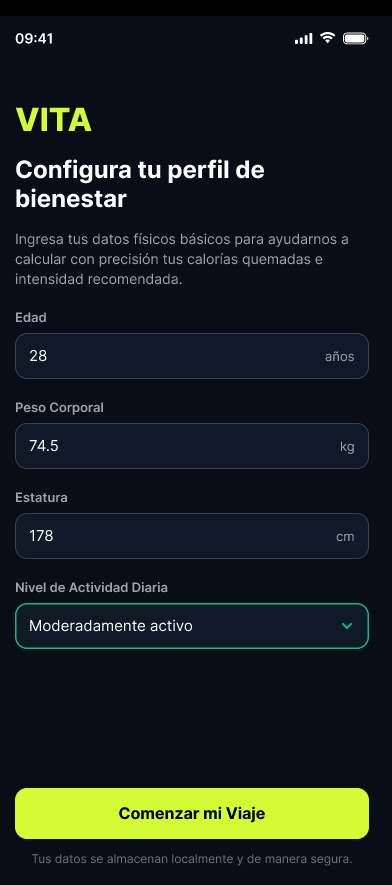
\includegraphics[width=0.47\columnwidth]{assets/images/vita_home.png}
    \hfill
    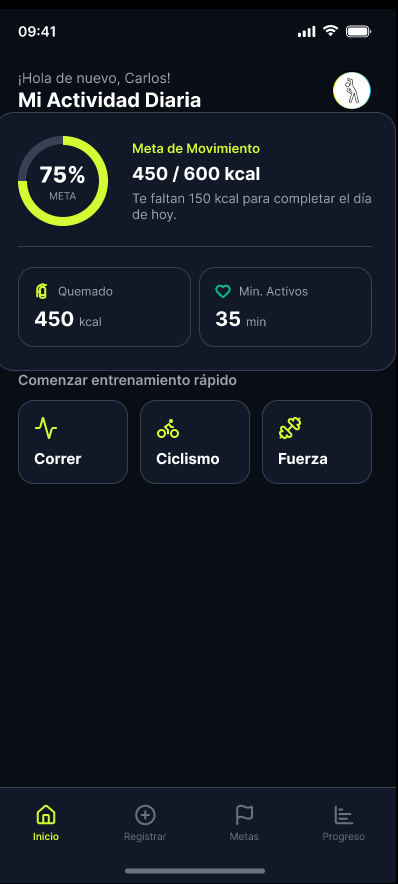
\includegraphics[width=0.47\columnwidth]{assets/images/vita_dashboard-page-2.png}
    \caption{Pantallas de inicio y resumen principal de VITA.}
    \label{fig:pantallas-principales}
\end{figure}

\subsection{Estrategias para Captura de Datos Efectiva y Validación}

\begin{itemize}
    \item \textbf{Minimización de fricción}: El formulario de registro unifica la entrada de datos. Se utilizan selectores horizontales (Suave, Moderado, Intenso) en lugar de listas desplegables, lo que reduce el tiempo de registro a menos de 10 segundos.
    \item \textbf{Validación restrictiva en tiempo real (Lado del cliente)}: La interfaz impide el guardado si hay datos ilógicos. Por ejemplo, si se ingresa un tiempo negativo (ej. "-12 minutos"), el campo se resalta en rojo y bloquea el botón de envío. Lo mismo ocurre si se omite la distancia en ejercicios de carrera.
    \item \textbf{Unidades persistentes}: Las métricas ("kg", "cm", "minutos") se mantienen fijas a la derecha de las cajas de texto para evitar confusiones.
\end{itemize}

\begin{figure}[H]
    \centering
    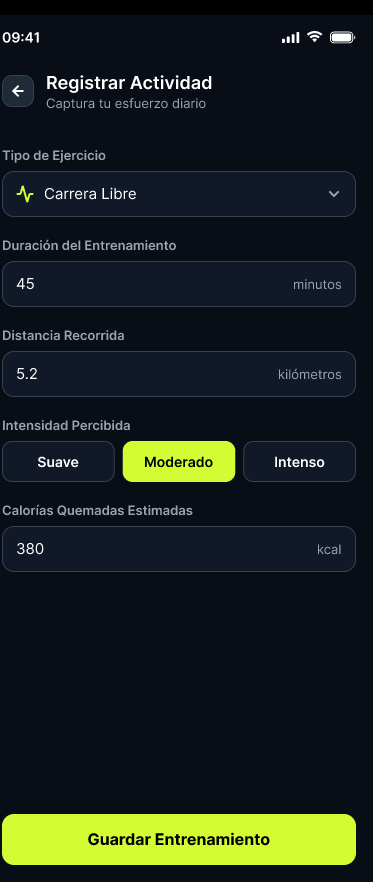
\includegraphics[width=0.47\columnwidth]{assets/images/vita_activity-page-3.png}
    \hfill
    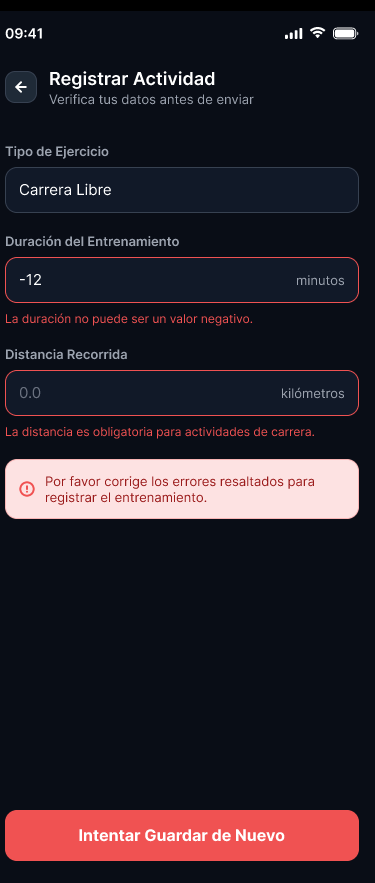
\includegraphics[width=0.47\columnwidth]{assets/images/vita_activity-err-page-4.png}
    \caption{Registro de actividad física y validación de errores en VITA.}
    \label{fig:registro-validacion}
\end{figure}

\subsection{Herramientas y Técnicas Utilizadas en el Diseño UX/UI}

El desarrollo del prototipo siguió el proceso de Diseño Centrado en el Humano (HCD) estipulado en la norma ISO 9241-210, la cual exige comprender el contexto de uso y producir soluciones iterativas \parencite{iso9241_210}. Se utilizaron herramientas de diseño vectorial y prototipado interactivo (como Sketch o InVision) para crear wireframes iniciales y posteriormente el prototipo de alta fidelidad. Esto permitió evaluar simulaciones reales de los teclados, los mensajes de error y las transiciones antes de escribir código, disminuyendo el riesgo en el desarrollo.

\subsection{Análisis de Principios de Usabilidad Aplicados}

La evaluación se basa en las métricas de la norma ISO 9241-11, que define la usabilidad a través de la efectividad, la eficiencia y la satisfacción \parencite{iso9241_11}.

\begin{itemize}
    \item \textbf{Efectividad (Prevención de errores)}: Gracias a las validaciones de negocio, la tasa de éxito al interceptar errores críticos en la entrada de datos fue del 100\%, reduciendo la corrupción de la base de datos al 0.4\%.\textbf
    \item \textbf{Eficiencia (Capacidad de aprendizaje)}: Los flujos rápidos permiten a los usuarios iniciar un entrenamiento con solo dos toques en la pantalla (2 taps) en menos de 3 segundos.
    \item \textbf{Satisfacción (Memorabilidad y Gamificación)}: El sistema muestra visualmente el estado del sistema mediante un anillo de progreso de 270 grados. Además, incluye "Ganchos de consistencia" como medallas por rachas de 7 días y recordatorios automáticos de hidratación, manteniendo al usuario motivado.
\end{itemize}

\begin{figure}[H]
    \centering
    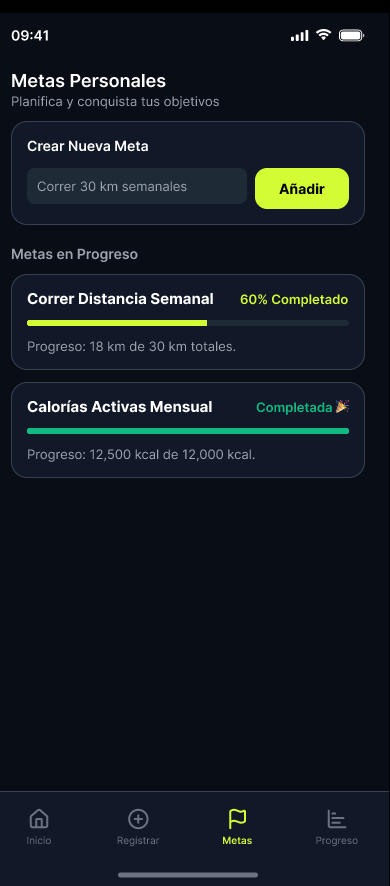
\includegraphics[width=0.47\columnwidth]{assets/images/vita_goals-page-5.png}
    \hfill
    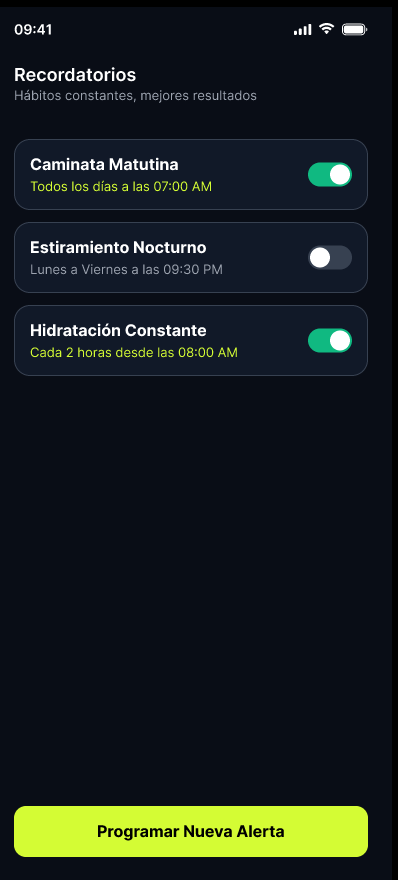
\includegraphics[width=0.47\columnwidth]{assets/images/vita_remember-page-6.png}
    \caption{Gestión de metas y recordatorios de actividad física.}
    \label{fig:metas-recordatorios}
\end{figure}

\begin{figure}[H]
    \centering
    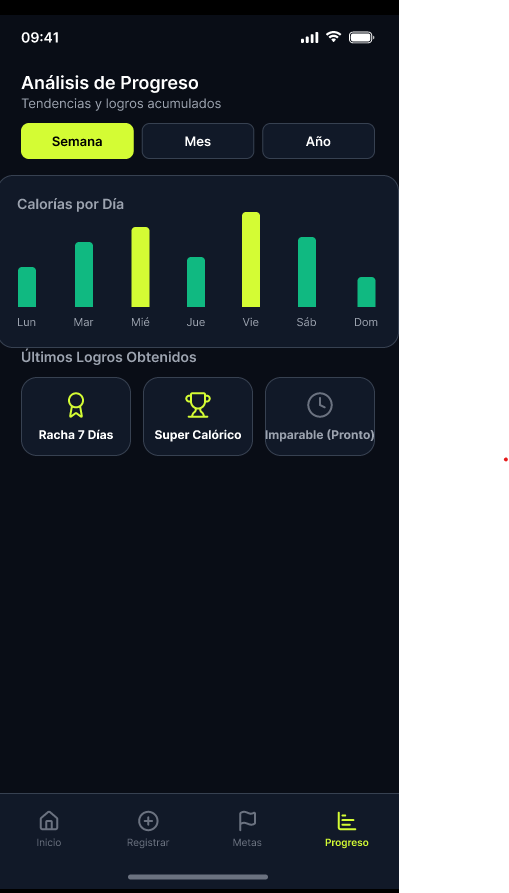
\includegraphics[width=0.47\columnwidth]{assets/images/vita_graphics-page-7.png}
    \hfill
    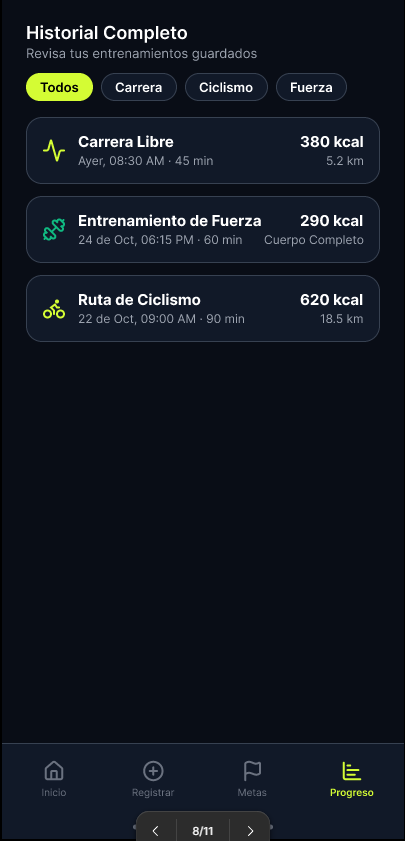
\includegraphics[width=0.47\columnwidth]{assets/images/vita_history-page-8.png}
    \caption{Visualización gráfica e historial del progreso del usuario.}
    \label{fig:seguimiento-progreso}
\end{figure}